\section{Results}
\label{sec:results}

The quantities used and the yield obtained are summarised in
Table~\ref{tab:yield}. The theoretical yield is based on salicylic acid as the
limiting reagent, with $M(\ce{C9H8O4}) = \SI{180.16}{\gram\per\mole}$:
\begin{equation}
  \text{yield} = \frac{m_\text{obs}}{n_\text{SA}\,M_\text{ASA}} \times 100
  = \frac{\SI{1.864}{\gram}}{\SI{14.49}{\milli\mole} \times \SI{180.16}{\gram\per\mole}}
  \times 100 = \SI{71.4}{\percent}
  \label{eq:yield}
\end{equation}

\begin{table}[H]
  \centering
  \caption{Reagents, product and yield.}
  \label{tab:yield}
  \begin{tabular}{l S[table-format=3.2] S[table-format=1.3] S[table-format=2.2]}
    \toprule
    {Compound} & {$M$ / \si{\gram\per\mole}} & {$m$ / \si{\gram}} & {$n$ / \si{\milli\mole}} \\
    \midrule
    Salicylic acid       & 138.12 & 2.002 & 14.49 \\
    Acetic anhydride     & 102.09 & 5.40  & 52.9  \\
    Aspirin (crude)      & 180.16 & 2.113 & 11.73 \\
    Aspirin (recryst.)   & 180.16 & 1.864 & 10.35 \\
    \bottomrule
  \end{tabular}
\end{table}

The TLC plate (silica, 1:1 ethyl acetate/hexane) is shown in
Figure~\ref{fig:tlc}. Retention factors were $R_f = 0.42$ for the product and
$R_f = 0.55$ for salicylic acid.

\begin{figure}[H]
  \centering
  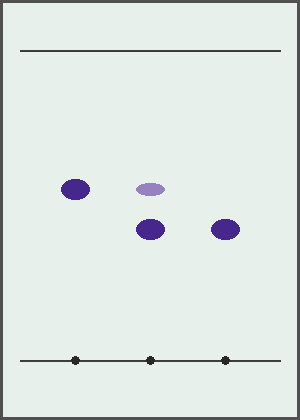
\includegraphics[width=0.4\textwidth]{tlc-plate.png}
  \caption{TLC plate under UV light: (1) salicylic acid, (2) crude product,
    (3) recrystallised product.}
  \label{fig:tlc}
\end{figure}

The measured melting point was \SIrange{134}{136}{\celsius} (literature
\SI{135}{\celsius}).
